\documentclass[twoside]{book}

% Packages required by doxygen
\usepackage{fixltx2e}
\usepackage{calc}
\usepackage{doxygen}
\usepackage[export]{adjustbox} % also loads graphicx
\usepackage{graphicx}
\usepackage[utf8]{inputenc}
\usepackage{makeidx}
\usepackage{multicol}
\usepackage{multirow}
\PassOptionsToPackage{warn}{textcomp}
\usepackage{textcomp}
\usepackage[nointegrals]{wasysym}
\usepackage[table]{xcolor}

% Font selection
\usepackage[T1]{fontenc}
\usepackage[scaled=.90]{helvet}
\usepackage{courier}
\usepackage{amssymb}
\usepackage{sectsty}
\renewcommand{\familydefault}{\sfdefault}
\allsectionsfont{%
  \fontseries{bc}\selectfont%
  \color{darkgray}%
}
\renewcommand{\DoxyLabelFont}{%
  \fontseries{bc}\selectfont%
  \color{darkgray}%
}
\newcommand{\+}{\discretionary{\mbox{\scriptsize$\hookleftarrow$}}{}{}}

% Page & text layout
\usepackage{geometry}
\geometry{%
  a4paper,%
  top=2.5cm,%
  bottom=2.5cm,%
  left=2.5cm,%
  right=2.5cm%
}
\tolerance=750
\hfuzz=15pt
\hbadness=750
\setlength{\emergencystretch}{15pt}
\setlength{\parindent}{0cm}
\setlength{\parskip}{3ex plus 2ex minus 2ex}
\makeatletter
\renewcommand{\paragraph}{%
  \@startsection{paragraph}{4}{0ex}{-1.0ex}{1.0ex}{%
    \normalfont\normalsize\bfseries\SS@parafont%
  }%
}
\renewcommand{\subparagraph}{%
  \@startsection{subparagraph}{5}{0ex}{-1.0ex}{1.0ex}{%
    \normalfont\normalsize\bfseries\SS@subparafont%
  }%
}
\makeatother

% Headers & footers
\usepackage{fancyhdr}
\pagestyle{fancyplain}
\fancyhead[LE]{\fancyplain{}{\bfseries\thepage}}
\fancyhead[CE]{\fancyplain{}{}}
\fancyhead[RE]{\fancyplain{}{\bfseries\leftmark}}
\fancyhead[LO]{\fancyplain{}{\bfseries\rightmark}}
\fancyhead[CO]{\fancyplain{}{}}
\fancyhead[RO]{\fancyplain{}{\bfseries\thepage}}
\fancyfoot[LE]{\fancyplain{}{}}
\fancyfoot[CE]{\fancyplain{}{}}
\fancyfoot[RE]{\fancyplain{}{\bfseries\scriptsize Generated by Doxygen }}
\fancyfoot[LO]{\fancyplain{}{\bfseries\scriptsize Generated by Doxygen }}
\fancyfoot[CO]{\fancyplain{}{}}
\fancyfoot[RO]{\fancyplain{}{}}
\renewcommand{\footrulewidth}{0.4pt}
\renewcommand{\chaptermark}[1]{%
  \markboth{#1}{}%
}
\renewcommand{\sectionmark}[1]{%
  \markright{\thesection\ #1}%
}

% Indices & bibliography
\usepackage{natbib}
\usepackage[titles]{tocloft}
\setcounter{tocdepth}{3}
\setcounter{secnumdepth}{5}
\makeindex

% Hyperlinks (required, but should be loaded last)
\usepackage{ifpdf}
\ifpdf
  \usepackage[pdftex,pagebackref=true]{hyperref}
\else
  \usepackage[ps2pdf,pagebackref=true]{hyperref}
\fi
\hypersetup{%
  colorlinks=true,%
  linkcolor=blue,%
  citecolor=blue,%
  unicode%
}

% Custom commands
\newcommand{\clearemptydoublepage}{%
  \newpage{\pagestyle{empty}\cleardoublepage}%
}

\usepackage{caption}
\captionsetup{labelsep=space,justification=centering,font={bf},singlelinecheck=off,skip=4pt,position=top}

%===== C O N T E N T S =====

\begin{document}

% Titlepage & ToC
\hypersetup{pageanchor=false,
             bookmarksnumbered=true,
             pdfencoding=unicode
            }
\pagenumbering{alph}
\begin{titlepage}
\vspace*{7cm}
\begin{center}%
{\Large S\+OG Pubquiz }\\
\vspace*{1cm}
{\large Generated by Doxygen 1.8.14}\\
\end{center}
\end{titlepage}
\clearemptydoublepage
\pagenumbering{roman}
\tableofcontents
\clearemptydoublepage
\pagenumbering{arabic}
\hypersetup{pageanchor=true}

%--- Begin generated contents ---
\chapter{pubquiz}
\label{md_README}
\Hypertarget{md_README}
studies without borders pubquiz scripting 
\chapter{Hierarchical Index}
\section{Class Hierarchy}
This inheritance list is sorted roughly, but not completely, alphabetically\+:\begin{DoxyCompactList}
\item \contentsline{section}{layout.\+Layout}{\pageref{classlayout_1_1Layout}}{}
\item \contentsline{section}{questions-\/simon.qround}{\pageref{classquestions-simon_1_1qround}}{}
\item \contentsline{section}{questions-\/simon.question}{\pageref{classquestions-simon_1_1question}}{}
\item \contentsline{section}{questions.\+questions}{\pageref{classquestions_1_1questions}}{}
\item \contentsline{section}{questions-\/simon.quiz}{\pageref{classquestions-simon_1_1quiz}}{}
\item Enum\begin{DoxyCompactList}
\item \contentsline{section}{layout.\+\_\+slide\+Index}{\pageref{classlayout_1_1__slideIndex}}{}
\end{DoxyCompactList}
\end{DoxyCompactList}

\chapter{Class Index}
\section{Class List}
Here are the classes, structs, unions and interfaces with brief descriptions\+:\begin{DoxyCompactList}
\item\contentsline{section}{\mbox{\hyperlink{classlayout_1_1__slideIndex}{layout.\+\_\+slide\+Index}} }{\pageref{classlayout_1_1__slideIndex}}{}
\item\contentsline{section}{\mbox{\hyperlink{classlayout_1_1Layout}{layout.\+Layout}} }{\pageref{classlayout_1_1Layout}}{}
\item\contentsline{section}{\mbox{\hyperlink{classquestions-simon_1_1qround}{questions-\/simon.\+qround}} }{\pageref{classquestions-simon_1_1qround}}{}
\item\contentsline{section}{\mbox{\hyperlink{classquestions-simon_1_1question}{questions-\/simon.\+question}} }{\pageref{classquestions-simon_1_1question}}{}
\item\contentsline{section}{\mbox{\hyperlink{classquestions_1_1questions}{questions.\+questions}} }{\pageref{classquestions_1_1questions}}{}
\item\contentsline{section}{\mbox{\hyperlink{classquestions-simon_1_1quiz}{questions-\/simon.\+quiz}} }{\pageref{classquestions-simon_1_1quiz}}{}
\end{DoxyCompactList}

\chapter{Class Documentation}
\hypertarget{classlayout_1_1__slideIndex}{}\section{layout.\+\_\+slide\+Index Class Reference}
\label{classlayout_1_1__slideIndex}\index{layout.\+\_\+slide\+Index@{layout.\+\_\+slide\+Index}}
Inheritance diagram for layout.\+\_\+slide\+Index\+:\begin{figure}[H]
\begin{center}
\leavevmode
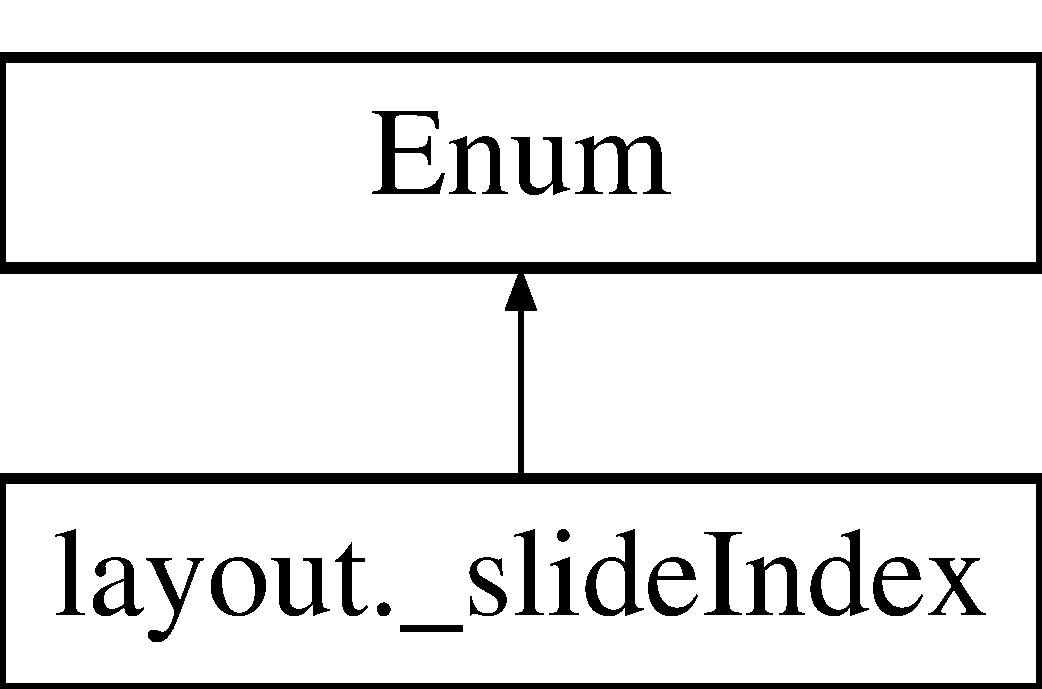
\includegraphics[height=2.000000cm]{classlayout_1_1__slideIndex}
\end{center}
\end{figure}
\subsection*{Static Public Attributes}
\begin{DoxyCompactItemize}
\item 
\mbox{\Hypertarget{classlayout_1_1__slideIndex_a7307216672fb3377c1b68ecce786d6f4}\label{classlayout_1_1__slideIndex_a7307216672fb3377c1b68ecce786d6f4}} 
int {\bfseries T\+I\+T\+L\+E\+\_\+\+S\+L\+I\+DE} = 0
\item 
\mbox{\Hypertarget{classlayout_1_1__slideIndex_a126f6d755cda24b09fd00b9eed497704}\label{classlayout_1_1__slideIndex_a126f6d755cda24b09fd00b9eed497704}} 
int {\bfseries S\+O\+G\+\_\+\+AD} = 1
\item 
\mbox{\Hypertarget{classlayout_1_1__slideIndex_ac8c6d7e6e65d65220ebfb3a1a56e3dfb}\label{classlayout_1_1__slideIndex_ac8c6d7e6e65d65220ebfb3a1a56e3dfb}} 
int {\bfseries R\+U\+L\+ES} = 2
\item 
\mbox{\Hypertarget{classlayout_1_1__slideIndex_a104bad61b57f6e8da41d1ab84dbd4e7c}\label{classlayout_1_1__slideIndex_a104bad61b57f6e8da41d1ab84dbd4e7c}} 
int {\bfseries Q\+U\+E\+S\+T\+I\+O\+N\+\_\+\+O\+P\+EN} = 3
\item 
\mbox{\Hypertarget{classlayout_1_1__slideIndex_a86d1e4e3338dff8fc55d98ad864f6da7}\label{classlayout_1_1__slideIndex_a86d1e4e3338dff8fc55d98ad864f6da7}} 
int {\bfseries Q\+U\+E\+S\+T\+I\+O\+N\+\_\+\+A\+L\+T\+E\+R\+N\+A\+T\+I\+VE} = 4
\end{DoxyCompactItemize}


The documentation for this class was generated from the following file\+:\begin{DoxyCompactItemize}
\item 
classes/layout.\+py\end{DoxyCompactItemize}

\hypertarget{classlayout_1_1Layout}{}\section{layout.\+Layout Class Reference}
\label{classlayout_1_1Layout}\index{layout.\+Layout@{layout.\+Layout}}
\subsection*{Public Member Functions}
\begin{DoxyCompactItemize}
\item 
\mbox{\Hypertarget{classlayout_1_1Layout_a7db96bc878fd1f07250baca76551d335}\label{classlayout_1_1Layout_a7db96bc878fd1f07250baca76551d335}} 
def {\bfseries \+\_\+\+\_\+init\+\_\+\+\_\+} (self, path\+Layout=file\+Name\+\_\+layout)
\item 
def \mbox{\hyperlink{classlayout_1_1Layout_a863963cd203ccb0d31fef73dc598f138}{get\+Title\+Slide}} (self)
\item 
def \mbox{\hyperlink{classlayout_1_1Layout_a3f7cfd8b7c1f699089e983e03398be91}{get\+S\+O\+Gadvertisement}} (self)
\end{DoxyCompactItemize}
\subsection*{Public Attributes}
\begin{DoxyCompactItemize}
\item 
\mbox{\Hypertarget{classlayout_1_1Layout_a798df89eacff80ee8fe674b32f3b2820}\label{classlayout_1_1Layout_a798df89eacff80ee8fe674b32f3b2820}} 
{\bfseries prs}
\end{DoxyCompactItemize}


\subsection{Detailed Description}
\begin{DoxyVerb}Used to get the Slides objects used as template
\end{DoxyVerb}
 

\subsection{Member Function Documentation}
\mbox{\Hypertarget{classlayout_1_1Layout_a3f7cfd8b7c1f699089e983e03398be91}\label{classlayout_1_1Layout_a3f7cfd8b7c1f699089e983e03398be91}} 
\index{layout\+::\+Layout@{layout\+::\+Layout}!get\+S\+O\+Gadvertisement@{get\+S\+O\+Gadvertisement}}
\index{get\+S\+O\+Gadvertisement@{get\+S\+O\+Gadvertisement}!layout\+::\+Layout@{layout\+::\+Layout}}
\subsubsection{\texorpdfstring{get\+S\+O\+Gadvertisement()}{getSOGadvertisement()}}
{\footnotesize\ttfamily def layout.\+Layout.\+get\+S\+O\+Gadvertisement (\begin{DoxyParamCaption}\item[{}]{self }\end{DoxyParamCaption})}

\begin{DoxyVerb}Get the slide used to show what is SOG
:return: Slide object
\end{DoxyVerb}
 \mbox{\Hypertarget{classlayout_1_1Layout_a863963cd203ccb0d31fef73dc598f138}\label{classlayout_1_1Layout_a863963cd203ccb0d31fef73dc598f138}} 
\index{layout\+::\+Layout@{layout\+::\+Layout}!get\+Title\+Slide@{get\+Title\+Slide}}
\index{get\+Title\+Slide@{get\+Title\+Slide}!layout\+::\+Layout@{layout\+::\+Layout}}
\subsubsection{\texorpdfstring{get\+Title\+Slide()}{getTitleSlide()}}
{\footnotesize\ttfamily def layout.\+Layout.\+get\+Title\+Slide (\begin{DoxyParamCaption}\item[{}]{self }\end{DoxyParamCaption})}

\begin{DoxyVerb}Get the slide used as the Title one, the first
:return: Slide object
\end{DoxyVerb}
 

The documentation for this class was generated from the following file\+:\begin{DoxyCompactItemize}
\item 
classes/layout.\+py\end{DoxyCompactItemize}

\hypertarget{classquestions-simon_1_1qround}{}\section{questions-\/simon.qround Class Reference}
\label{classquestions-simon_1_1qround}\index{questions-\/simon.\+qround@{questions-\/simon.\+qround}}
\subsection*{Public Member Functions}
\begin{DoxyCompactItemize}
\item 
\mbox{\Hypertarget{classquestions-simon_1_1qround_a47efe77bf526cb5367f784dfc7c77d60}\label{classquestions-simon_1_1qround_a47efe77bf526cb5367f784dfc7c77d60}} 
def {\bfseries add\+Question} (Self, \mbox{\hyperlink{classquestions-simon_1_1question}{question}})
\item 
\mbox{\Hypertarget{classquestions-simon_1_1qround_af59b9832be8715c62c25a51987767eb6}\label{classquestions-simon_1_1qround_af59b9832be8715c62c25a51987767eb6}} 
def {\bfseries dump} (Self)
\end{DoxyCompactItemize}
\subsection*{Static Public Attributes}
\begin{DoxyCompactItemize}
\item 
\mbox{\Hypertarget{classquestions-simon_1_1qround_af36752e2648863329a600dea111547ad}\label{classquestions-simon_1_1qround_af36752e2648863329a600dea111547ad}} 
list {\bfseries questions} = \mbox{[}$\,$\mbox{]}
\end{DoxyCompactItemize}


The documentation for this class was generated from the following file\+:\begin{DoxyCompactItemize}
\item 
classes/questions-\/simon.\+py\end{DoxyCompactItemize}

\hypertarget{classquestions-simon_1_1question}{}\section{questions-\/simon.question Class Reference}
\label{classquestions-simon_1_1question}\index{questions-\/simon.\+question@{questions-\/simon.\+question}}
\subsection*{Public Member Functions}
\begin{DoxyCompactItemize}
\item 
\mbox{\Hypertarget{classquestions-simon_1_1question_ad81487e067da563aed36fd2fdf42fe99}\label{classquestions-simon_1_1question_ad81487e067da563aed36fd2fdf42fe99}} 
def {\bfseries \+\_\+\+\_\+init\+\_\+\+\_\+} (Self, q)
\item 
\mbox{\Hypertarget{classquestions-simon_1_1question_af8dfc02000d09bd7408573c38b97de56}\label{classquestions-simon_1_1question_af8dfc02000d09bd7408573c38b97de56}} 
def {\bfseries add\+Answer} (Self, answer, correct)
\item 
\mbox{\Hypertarget{classquestions-simon_1_1question_abcab6d7d7f0e282314a3577dbbcf1a28}\label{classquestions-simon_1_1question_abcab6d7d7f0e282314a3577dbbcf1a28}} 
def {\bfseries set\+Image} (Self, image)
\item 
\mbox{\Hypertarget{classquestions-simon_1_1question_ad6d346c4b9ebdbd0ccf2cd93c1042126}\label{classquestions-simon_1_1question_ad6d346c4b9ebdbd0ccf2cd93c1042126}} 
def {\bfseries get\+Image} (Self)
\item 
\mbox{\Hypertarget{classquestions-simon_1_1question_a974643d89fa5caeb901ba799cae4bce1}\label{classquestions-simon_1_1question_a974643d89fa5caeb901ba799cae4bce1}} 
def {\bfseries set\+Comment} (Self, comment)
\item 
\mbox{\Hypertarget{classquestions-simon_1_1question_a3fe81e28952d76e488aab9939567b008}\label{classquestions-simon_1_1question_a3fe81e28952d76e488aab9939567b008}} 
def {\bfseries get\+Comment} (Self)
\item 
\mbox{\Hypertarget{classquestions-simon_1_1question_a87f633095bf96a8f88122821110c9ab8}\label{classquestions-simon_1_1question_a87f633095bf96a8f88122821110c9ab8}} 
def {\bfseries dump} (Self)
\end{DoxyCompactItemize}
\subsection*{Static Public Attributes}
\begin{DoxyCompactItemize}
\item 
\mbox{\Hypertarget{classquestions-simon_1_1question_ac82eef3a0c80e949ff36a0ab59a1165d}\label{classquestions-simon_1_1question_ac82eef3a0c80e949ff36a0ab59a1165d}} 
string {\bfseries question} = \char`\"{}\char`\"{}
\item 
\mbox{\Hypertarget{classquestions-simon_1_1question_a086ac1191ad5f1cf3b4fc1b60f93e838}\label{classquestions-simon_1_1question_a086ac1191ad5f1cf3b4fc1b60f93e838}} 
dictionary {\bfseries answers} = \{\}
\end{DoxyCompactItemize}


The documentation for this class was generated from the following file\+:\begin{DoxyCompactItemize}
\item 
classes/questions-\/simon.\+py\end{DoxyCompactItemize}

\hypertarget{classquestions_1_1questions}{}\section{questions.\+questions Class Reference}
\label{classquestions_1_1questions}\index{questions.\+questions@{questions.\+questions}}
\subsection*{Public Member Functions}
\begin{DoxyCompactItemize}
\item 
\mbox{\Hypertarget{classquestions_1_1questions_aabcabf708dce7cfcdf04020e2617f725}\label{classquestions_1_1questions_aabcabf708dce7cfcdf04020e2617f725}} 
def {\bfseries \+\_\+\+\_\+init\+\_\+\+\_\+} (self)
\item 
\mbox{\Hypertarget{classquestions_1_1questions_a8814d385d95b740c575bb3b6c6ef7da6}\label{classquestions_1_1questions_a8814d385d95b740c575bb3b6c6ef7da6}} 
def {\bfseries read\+All\+Csv\+Files} (self)
\end{DoxyCompactItemize}


The documentation for this class was generated from the following file\+:\begin{DoxyCompactItemize}
\item 
classes/questions.\+py\end{DoxyCompactItemize}

\hypertarget{classquestions-simon_1_1quiz}{}\section{questions-\/simon.quiz Class Reference}
\label{classquestions-simon_1_1quiz}\index{questions-\/simon.\+quiz@{questions-\/simon.\+quiz}}
\subsection*{Public Member Functions}
\begin{DoxyCompactItemize}
\item 
\mbox{\Hypertarget{classquestions-simon_1_1quiz_a36a2cfa78434336af8dec943bc8d4b1b}\label{classquestions-simon_1_1quiz_a36a2cfa78434336af8dec943bc8d4b1b}} 
def {\bfseries add\+Round} (Self, rnd)
\item 
\mbox{\Hypertarget{classquestions-simon_1_1quiz_a6af12da1b218f3a7f6d43126fe2f94e3}\label{classquestions-simon_1_1quiz_a6af12da1b218f3a7f6d43126fe2f94e3}} 
def {\bfseries dump} (Self)
\end{DoxyCompactItemize}
\subsection*{Static Public Attributes}
\begin{DoxyCompactItemize}
\item 
\mbox{\Hypertarget{classquestions-simon_1_1quiz_a2b862c6463d392925b4f6b1f1d5e5ba6}\label{classquestions-simon_1_1quiz_a2b862c6463d392925b4f6b1f1d5e5ba6}} 
list {\bfseries rounds} = \mbox{[}$\,$\mbox{]}
\end{DoxyCompactItemize}


The documentation for this class was generated from the following file\+:\begin{DoxyCompactItemize}
\item 
classes/questions-\/simon.\+py\end{DoxyCompactItemize}

%--- End generated contents ---

% Index
\backmatter
\newpage
\phantomsection
\clearemptydoublepage
\addcontentsline{toc}{chapter}{Index}
\printindex

\end{document}
